\documentclass[tikz,border=2pt]{standalone}
\usepackage{amsmath}
\usepackage{pgfplots}
\pgfplotsset{compat=1.18}

\begin{document}
% a_n <= b_n <= c_n with a_n and c_n both tending to L: the middle sequence is trapped and
% must tend to L as well.
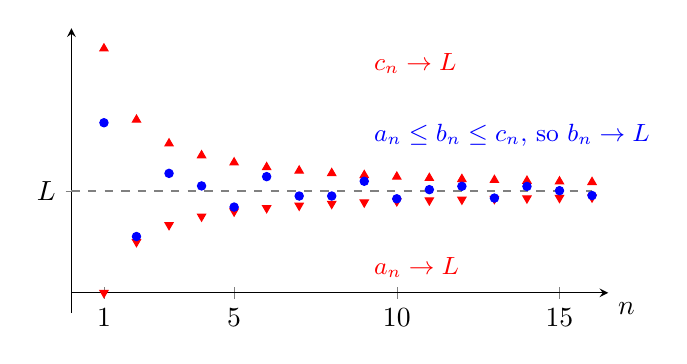
\begin{tikzpicture}
	\begin{axis}[
		axis lines=middle,
		xmin=0, xmax=16.5,
		ymin=-0.2, ymax=2.6,
		xtick={1,5,10,15}, ytick={1}, yticklabels={$L$},
		xlabel={$n$}, ylabel={},
		xlabel style={below right},
		clip=false,
		width=8.4cm, height=5.2cm
		]
		\addplot[gray, dashed, domain=0:16] {1};
		\addplot[only marks, mark=triangle*, mark size=1.7pt, red, samples at={1,...,16}] {1+1.4/x};
		\addplot[only marks, mark=triangle*, mark size=1.7pt, red, mark options={rotate=180}, samples at={1,...,16}] {1-1.0/x};
		\addplot[only marks, mark=*, mark size=1.5pt, blue, samples at={1,...,16}] {1+0.9*sin(deg(2.3*x))/x};
		\node[red, anchor=west, font=\small] at (axis cs:9,2.25) {$c_n\to L$};
		\node[red, anchor=west, font=\small] at (axis cs:9,0.25) {$a_n\to L$};
		\node[blue, anchor=west, font=\small] at (axis cs:9,1.55) {$a_n\le b_n\le c_n$, so $b_n\to L$};
	\end{axis}
\end{tikzpicture}
\end{document}
